\null\newpage
\section{Tieftöner- und Hochtönerweiche}\label{kap:5.2}
\subsection{Allgemeines}\label{kap:5.2.1}
Für die Satellitenlautsprecher, welche aus einem Hochtöner und einem Tieftöner bestehen werden nun die Teilfrequenzbereiche Mitte und Hoch benötigt. Da es sich bei dem Satellitensystem um ein Paar an Boxen handelt und diese räumlichen weiter entfernt voneinander stehen, können nun Stereo-Effekte verwendet und mit dem reinen Stereo-Eingangssignal gearbeitet werden. Eine Aufteilung des Signals in Linke- und Rechte-Satellitenbox muss jedoch schon getroffen werden, um die Effekte richtig zu erhalten. Dafür wird einfach für die Linke-Satellitenbox, bestehend aus Hoch- und Tieftöner die entsprechenden Weichen verwendet und das Selbe für die Rechte-Box.

\subsection{Zielsetzung}\label{kap:5.2.2}
Das unberührte Eingangssignal soll so gefiltert werden, dass der Hochtöner nur Frequenzen über 1,5kHz und der Tieftöner Frequenzen bis 6kHz zum abstrahlen erhält. Dementsprechend sollen die Filter gewählt und designet werden.\\
Obwohl es den Mono-Bass gibt der die untersten Frequenzen (>20Hz) abzustrahlen hat, dürfen die Satelliten-Tieftöner im selbigen Bereich ebenfalls spielen. Somit wird die abstrahlende Fläche vergrößert und freiwerdende absolute Pegel höher. Bei dem Satelliten-Tieftöner wird jedoch ein Bandpass vorgesehen um bei möglichen Resonanzen mit dem Mono-Bass das Signal filtern zu können.\\
Dementsprechend sollen die Filter gewählt und designet werden.

\subsection{Filter}\label{kap:5.2.3}
Es wurden wie bereits in Kapitel \ref{kap:5.1} \enquote{Butterworth-Tiefpass-Filter 2. Ordnung} verwendet. Dieses mal ein Bandpass-Filter und ein Hochpass-Filter ebenfalls nach Butterworth. Dabei handelt es sich wieder um \enquote{Aktive-Filter} was bedeutet, dass OPV-Schaltungen verwendet wurden.\\
Das Bandpass-Filter(\ref{fig:abb5.2.3.1}) besteht aus drei Widerständen, zwei Kondensatoren und einem OPV dieser wird am Minus-Eingang angesteuert was zur folge hat, dass die Schaltung invertierend wirkt was aber keine Probleme aufbringt. Am Plus-Eingang des OPVs wird entweder Masse bei symmetrische Versorgungsspannung oder $\frac{Vcc}{2}$ bei asymmetrischer verwendet.
\begin{figure} [H]
	\centering
	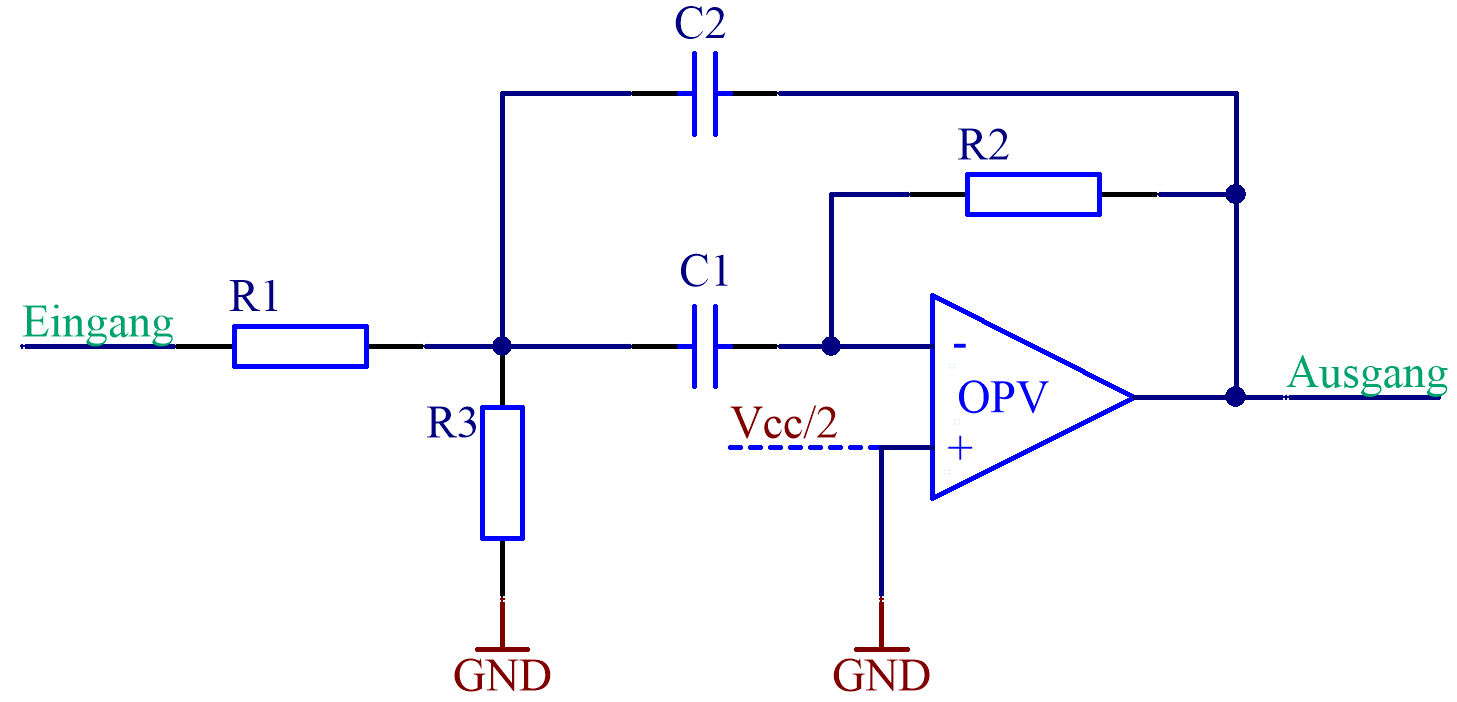
\includegraphics[width=1\textwidth]{img/Print4/BPFilter-Butterworth2Ordnung.PNG}
	\caption{Butterworth-Bandpass-Filter 2. Ordnung}
	\label {fig:abb5.2.3.1}
\end{figure}
Ähnliche Konstruktion hat der Hochpass(\ref{fig:abb5.2.3.2}). Dieser besteht aus drei Kondensatoren, zwei Widerständen und einem OPV.\\
\begin{figure} [H]
	\centering	
	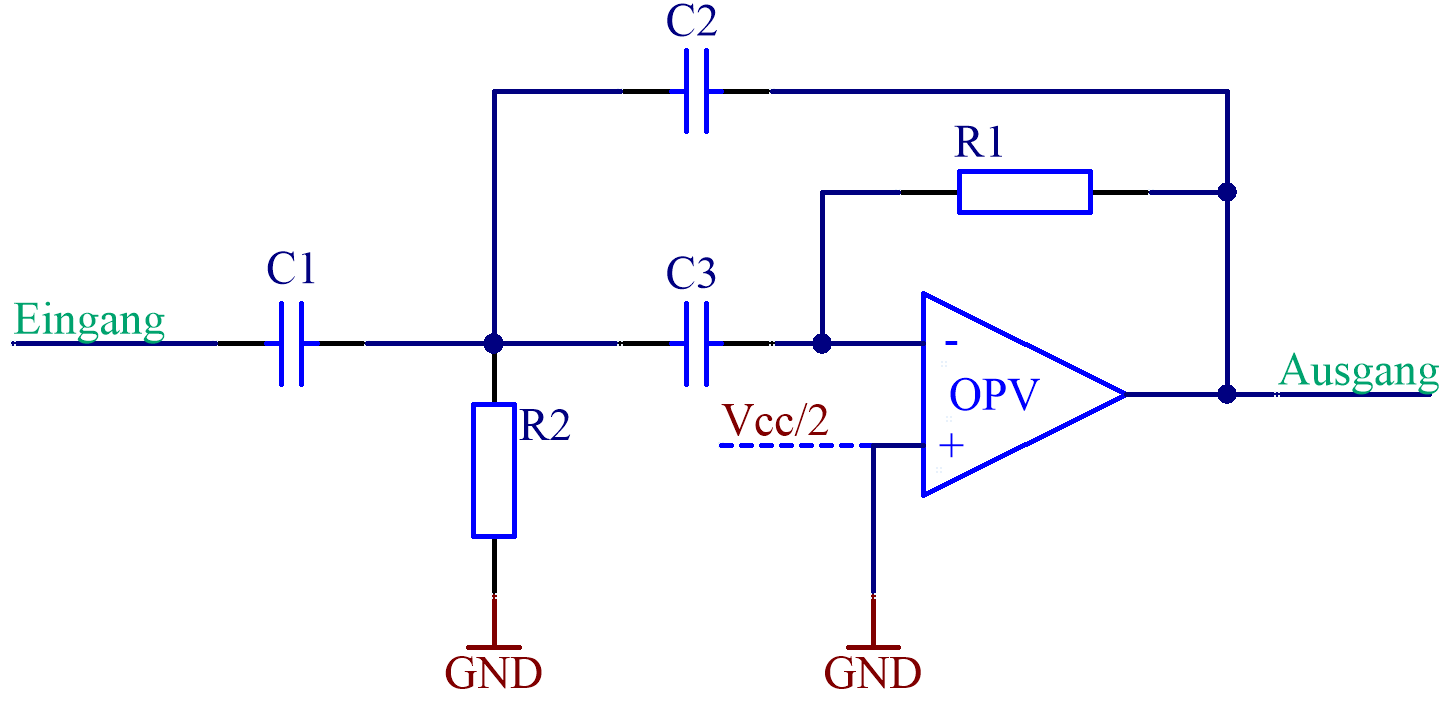
\includegraphics[width=1\textwidth]{img/Print4/HPFilter-Butterworth2Ordnung.PNG}
	\caption{Butterworth-Hochpass-Filter 2. Ordnung}
	\label {fig:abb5.2.3.2}
\end{figure}

\subsection{Schaltung}\label{kap:5.2.4}

Das Eingangssignal (Links, Rechts, Masse) wird an einer dreipoligen Stifleiste angeschlosssen (Abb. \ref{fig:abb5.2.4.1}). Zuerst gelangt Signal-Links und -Rechts an jeweils ein Potentiometer um den Pegel anpassen zu können, es bietet also eine Regelmöglichkeit. Es folgen die Filter. Hochpass für Links/Rechts und Tiefpass für Links/Rechts. Ein \enquote{Butterworth-Tiefpass-Filter 2. Ordnung} wurde bereits in dem Kapitel \ref{kap:5.1.4} erklärt. Das \enquote{Butterworth-Hochpass-Filter und -Bandpass-Filter 2. Ordnung} weist keine groben Unterschiede auf, der Unterschied liegt lediglich in der Bauteilaufteilung.\\
Nach den Filtern gelangen die getrennten Signale zu deren Ausgangspunkt. Es ist für jede Signalleitung eine zweipolige Stiftleist vorgesehen (Signal + Masse), da der darauffolgende Verstärker einen selbigen Eingang besitzt. Die Stiftleisten sind jedoch gruppiert nach Bandpass- und Hochpass-Ausgang.\\
\begin{figure} [H]
	\centering	
	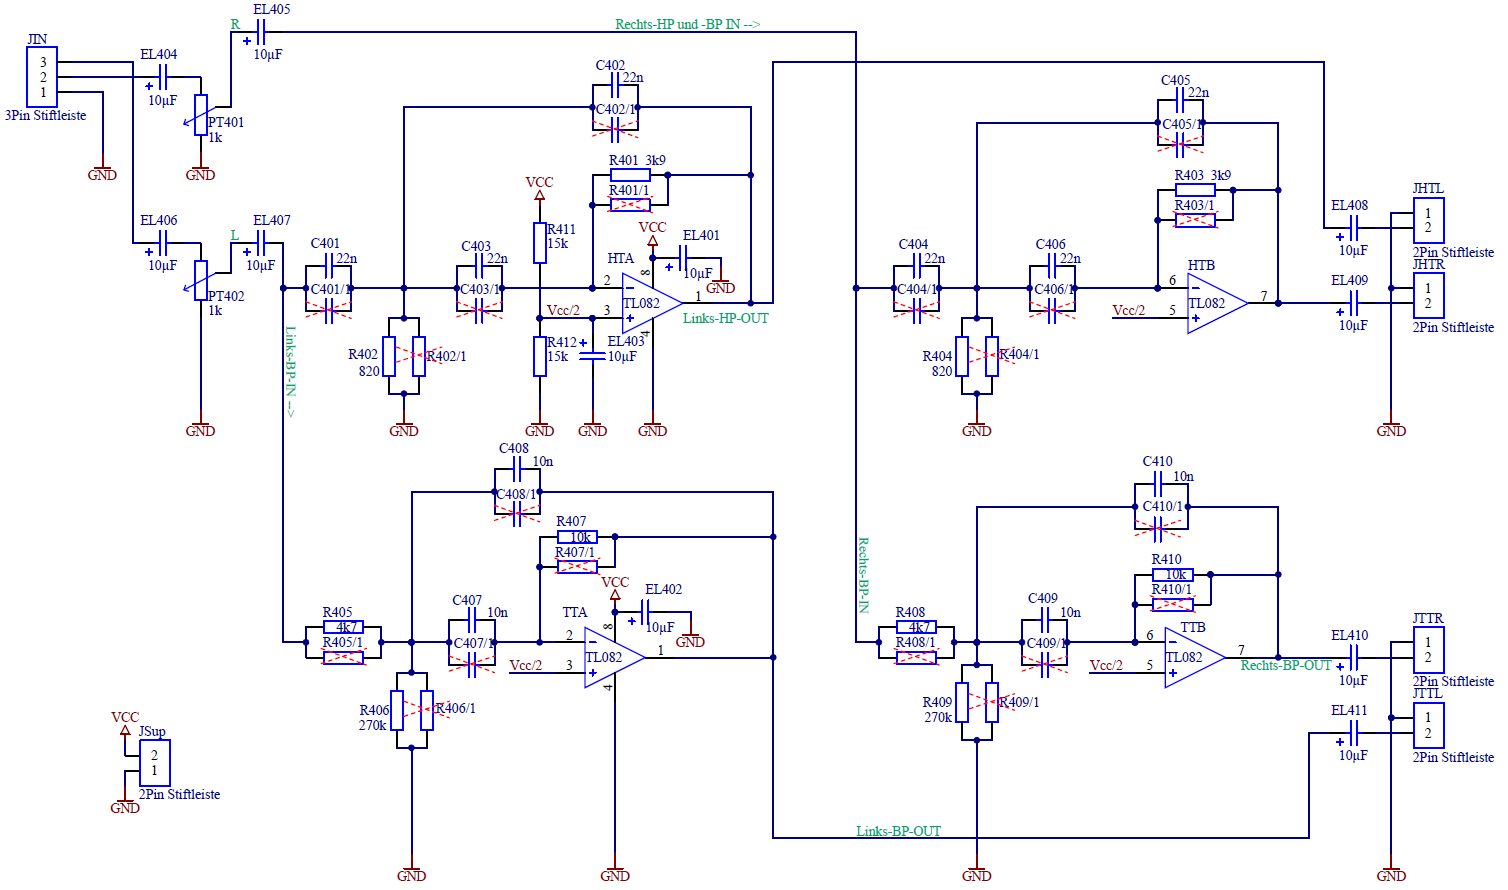
\includegraphics[width=1\textwidth]{img/Print4/4_TTuHTWeiche-Schematic.PNG}
	\caption{Butterworth-Bandpass-Filter 2. Ordnung}
	\label {fig:abb5.2.4.1}
\end{figure}
Eines der Bandpass-Filter. Gut sichtbar die doppelte, parallele Ausführung von Widerständen und Kondensatoren um krumme Werte auch erhalten zu können. Bedingt durch Parallel-Schaltung von Widerständen und Kondensatoren.\\ 
Der Eingang wurde gespiegelt um ein schöneres Bild zu erlangen. Die Spiegelung ist für das PCB-Layout nicht relevant!\\
Bedingt durch die Versorgungsspannung ist auch der Spannungsteiler für $\frac{Vcc}{2}$ am Plus-Eingang des OPVs implementiert.
\begin{figure} [H]
	\centering	
	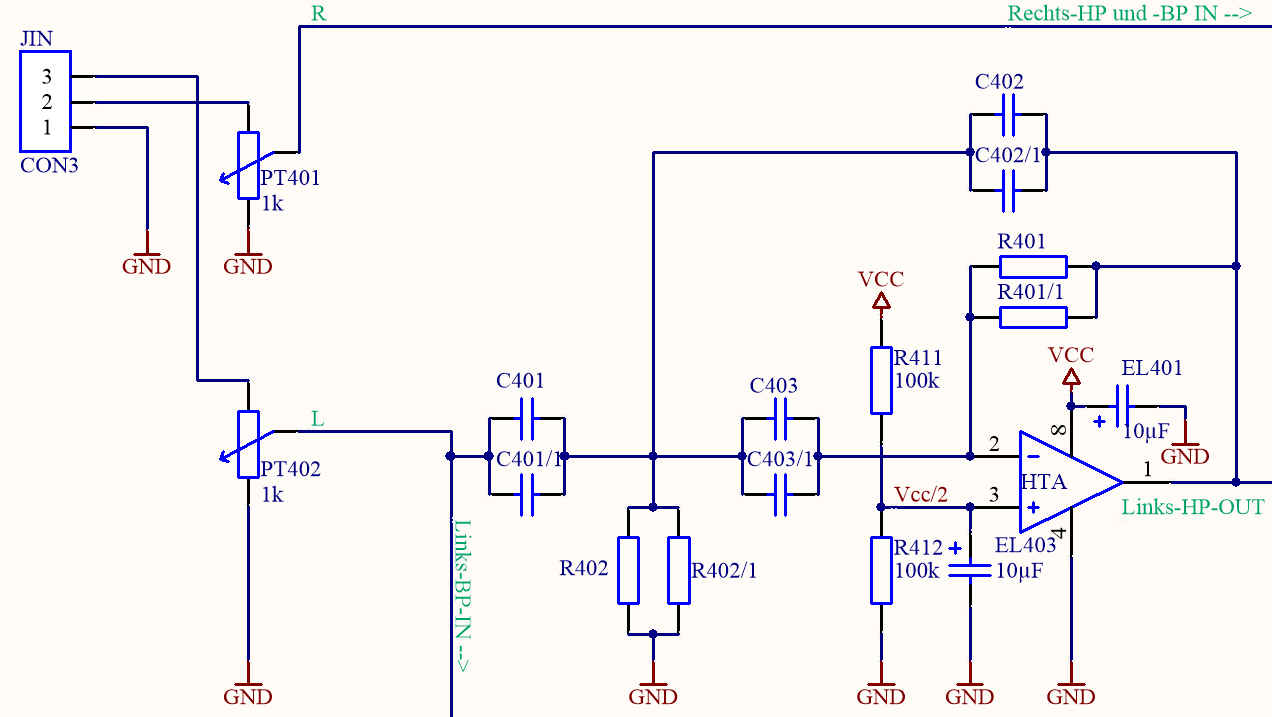
\includegraphics[width=1\textwidth]{img/Print4/4_TTuHTWeiche-LinksHP-Schematic.PNG}
	\caption{Butterworth-Bandpass-Filter 2. Ordnung - aus Abb.\ref{fig:abb5.2.4.1}}
	\label {fig:abb5.2.4.2}
\end{figure}
Am B-Teil des OPVs (erkennbar an der Beschriftung: TT\enquote{B}) ist keine Versorgung einzuzeichnen, da er mit dem A-Teil einen achtpinnigen IC mit zwei integrierten OPVs ergibt. Die zwei Teile sind über das IC-Gehäuse mit der gleichen Versorgungsspannung verbunden, deshalb ist das einmalige Kennzeichnen ausreichend.\\
\begin{figure} [H]
	\centering	
	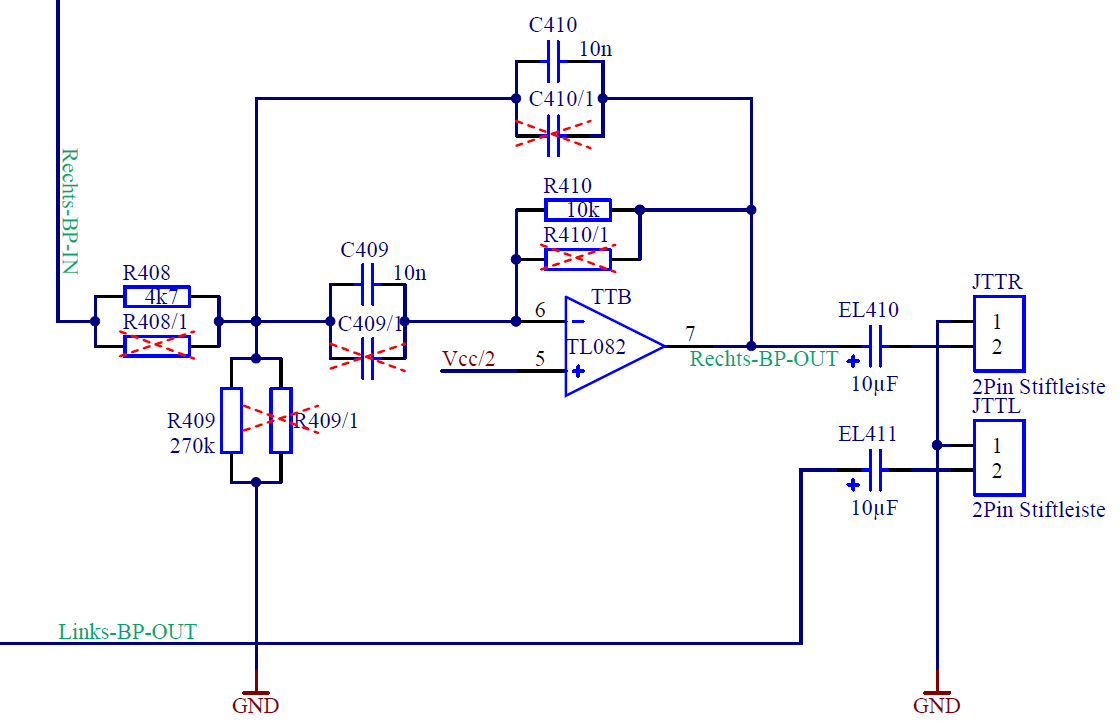
\includegraphics[width=1\textwidth]{img/Print4/4_TTuHTWeiche-RechtsBP-Schematic.PNG}
	\caption{Butterworth-Bandpass-Filter 2. Ordnung - aus Abb.\ref{fig:abb5.2.4.1}}
	\label {fig:abb5.2.4.3}
\end{figure}

\subsection{PCB}\label{kap:5.2.5}
Es wurden die grundlegenden Regeln zur Leiterplattenentflechtung angewandt (\ref{}). Bei dem Design (Abb. \ref{fig:abb5.2.5.1}) wurde auf hohe Variierbarkeit geachtet um auch zB. Kondensatoren mit unterschiedlichen Footprint verwenden zu können.\\
Es wurden wieder nahe an den IC's ELKOs in der Spannungsversorgungsleitung verbaut, um Störungen zu verhindern.

\begin{figure} [H]
	\centering	
	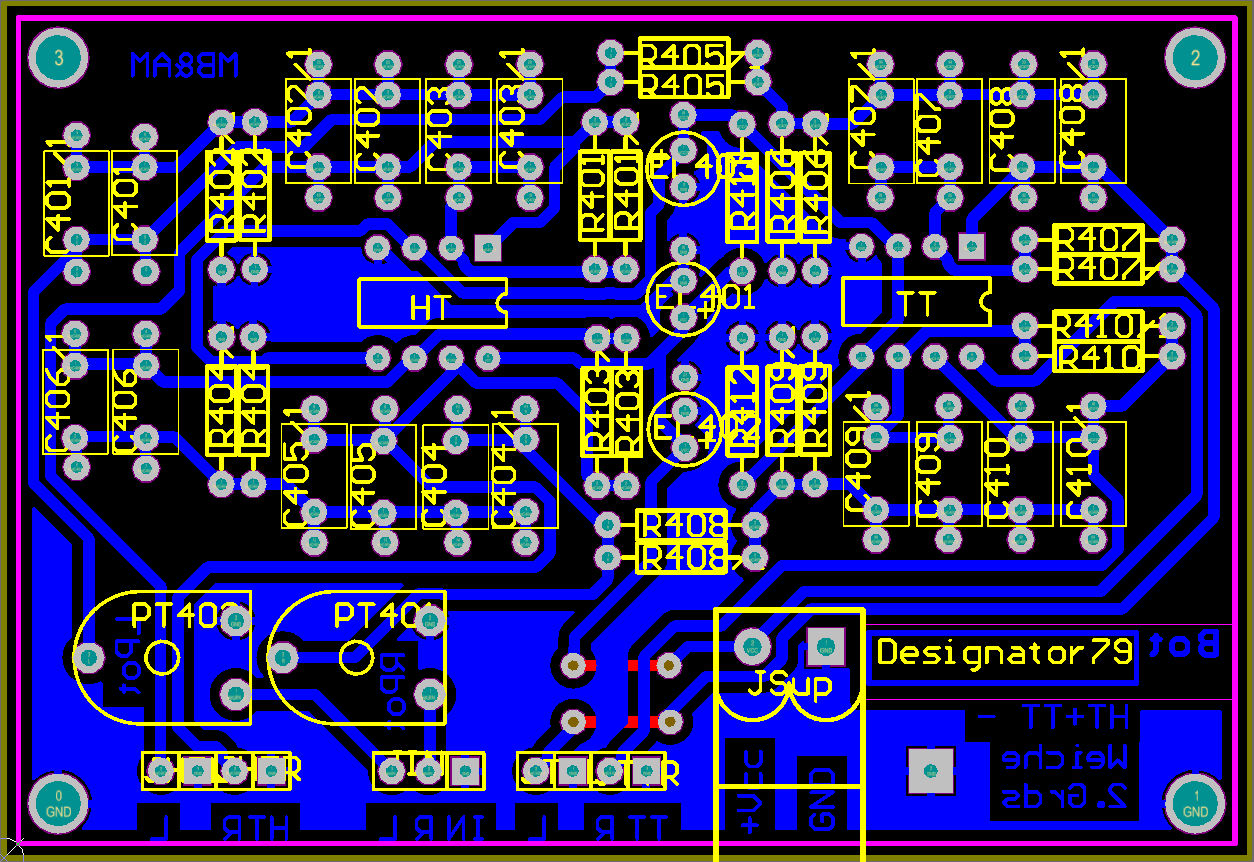
\includegraphics[width=1\textwidth]{img/Print4/4_TTuHTWeiche-PCB.PNG}
	\caption{Tieftöner- und Hochtönerweichen - PCB}
	\label {fig:abb5.2.5.1}
\end{figure}


\begin{comment}
%% Altium und Einstellungserklärung + Wichtige Layout-Faktoren
%Beim designen des Leiterplattenlayouts wurden die allgemeinen Altium-Einstellungen vorgenommen und auf die zu berücksichtigenden Layoutpunkte geachtet.
Beim \enquote{Layouten} der Schaltung mussten einige wichtige Faktoren berücksichtigt werden.\\
Wie da wären:\\
\begin{itemize}
	\item EMV-Technische-Faktoren, wie kurze Leiterbahnen
	\item Ausnützen der Printfläche
	\item Mehrfach-Footprints ermöglichen für verschiedene Bauteile
	\item Mechanische Aufhängebohrungen vorsehen
	\item Massefläche bei Möglichkeit vorsehen
\end{itemize}
Leiterplattenspezifische Einstellungen wurden aus den Kriterien der schuleigenen Leiterplattenfertigung übernommen. Zu diesen Einstellungen zählen:\\
\begin{itemize}
	\item Leiterbahnbreite
	\item Leiterbahnabstände untereinander
	\item Restring bei Bohrungen
	\item 
\end{itemize}

\subsection{Inbetriebnahme}
Bereits mit einer simplen Beschaltung kann das Modul in Betrieb genommen werden:
\begin{figure} [h]
	\centering
	\caption{Prinzipschaltung XS3868}
	\label {fig:abb2.3}
%%	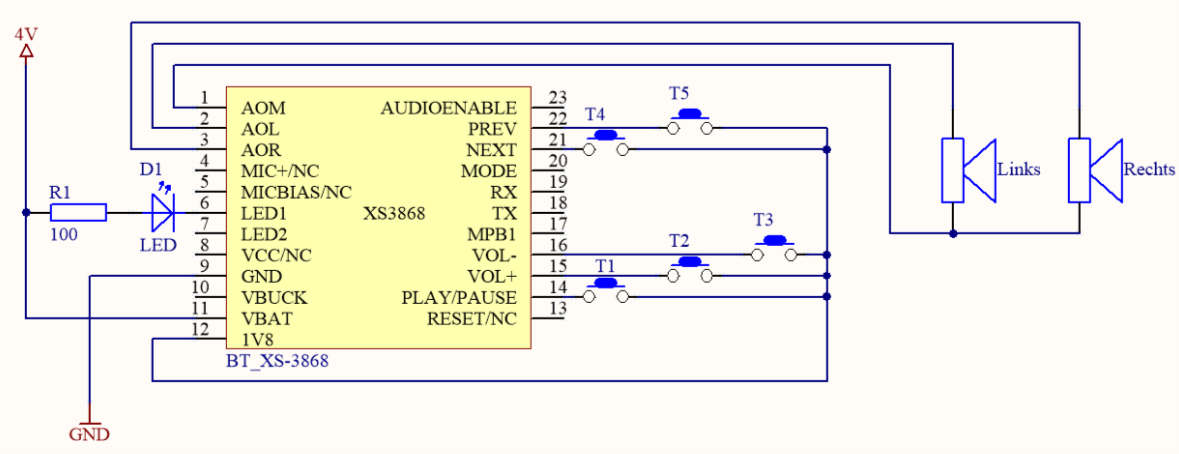
\includegraphics[width=1\textwidth]{schaltungen/XS3868_Prinzipschaltung.png}
\end{figure} \\
Mit dieser Schaltung (Abb. \ref {fig:abb2.3}) kann das Modul bereits ordnungsgemäß arbeiten.\\
Die Versorgungsspannung ist mit 4V etwas höher gewählt damit es nicht zu Ausfällen durch Spannungsschwankungen kommt. Das XS3868-Modul hat eine Stromaufnahme von ca. 30mA beim Starten, 10mA im Stand-By und bis zu 100mA wenn Musik abgespielt wird.\\ \\
Die Status-LED ist, wie in Abbildung \ref {fig:abb2.3} dargestellt, \enquote{Low-Aktiv}. Beim Starten des Moduls und während der Suche nach Geräten blinkt sie durchgehend, wobei sie bei einer bestehenden Verbindung nur die Hälfte der Zeit blinkt.\\ \\
Mit einfachem Betätigen eines Tasters wird die entsprechende Funktion vom Modul ausgeführt, jeweils mit einem Bestätigungston begleitet. Dieser Ton wird auch beim Starten des Moduls abgespielt.\\ \\
Statt die Lautsprecher direkt an das Modul anzuschließen, sollte allerdings noch ein Verstärker verbaut werden.
\newpage


\subsection{Verbindung mit dem Modul}
Wenn der OVC3860 eingeschaltet ist, sucht er andauernd nach BT-Geräten. Mit einem Smartphone findet man das Gerät und kann sich mit einem Standard-PIN-Code (\enquote{0000}) verbinden. Wenn bereits Lautsprecher angeschlossen sind, wird ein Ton abgespielt, der die Verbindung bestätigt. Außerdem hat die Status-LED nun ein anderes Blinkverhalten (Mehrmaliges Blinken mit längeren Pausen).\\ \\
Jetzt ist das Modul bereit Musik abzuspielen. Diese kann vom Smartphone oder vom Modul aus gesteuert werden. Die notwendigen Taster müssen allerdings schon in der Schaltung verbaut sein um die Bedienung der Musik zu ermöglichen.


\subsection{Zusatz-Leiterplatten}
\subsubsection{Allgemeines}
Als Entwicklungsprogramm für beide Leiterplatten wurde  \enquote{Altium Designer 13.3} verwendet. Die Schaltung wurde in diesem Programm gezeichnet, das Layout für die Leiterplatten angefertigt und entflechtet. Es wurden einseitige Platinen verwendet, da doppelseitige nicht notwendig waren.


\subsubsection{Adapter-Board}
Da das Modul in SMD-Bauform gefertigt ist, wurde ein Adapter-Board (Abb. \ref{fig:abb3.1}) vorgesehen um eine einfachere Handhabung mit dem Modul zu ermöglichen. Als Anschlussmöglichkeiten werden Stiftleisten verwendet.\\
Die Schaltung ist deshalb auch sehr simpel aufgebaut:
\begin{figure} [h]
	\centering
	\caption{Schaltung des Adapter-Boards}
	%%\label {fig:abb3.1}
%%	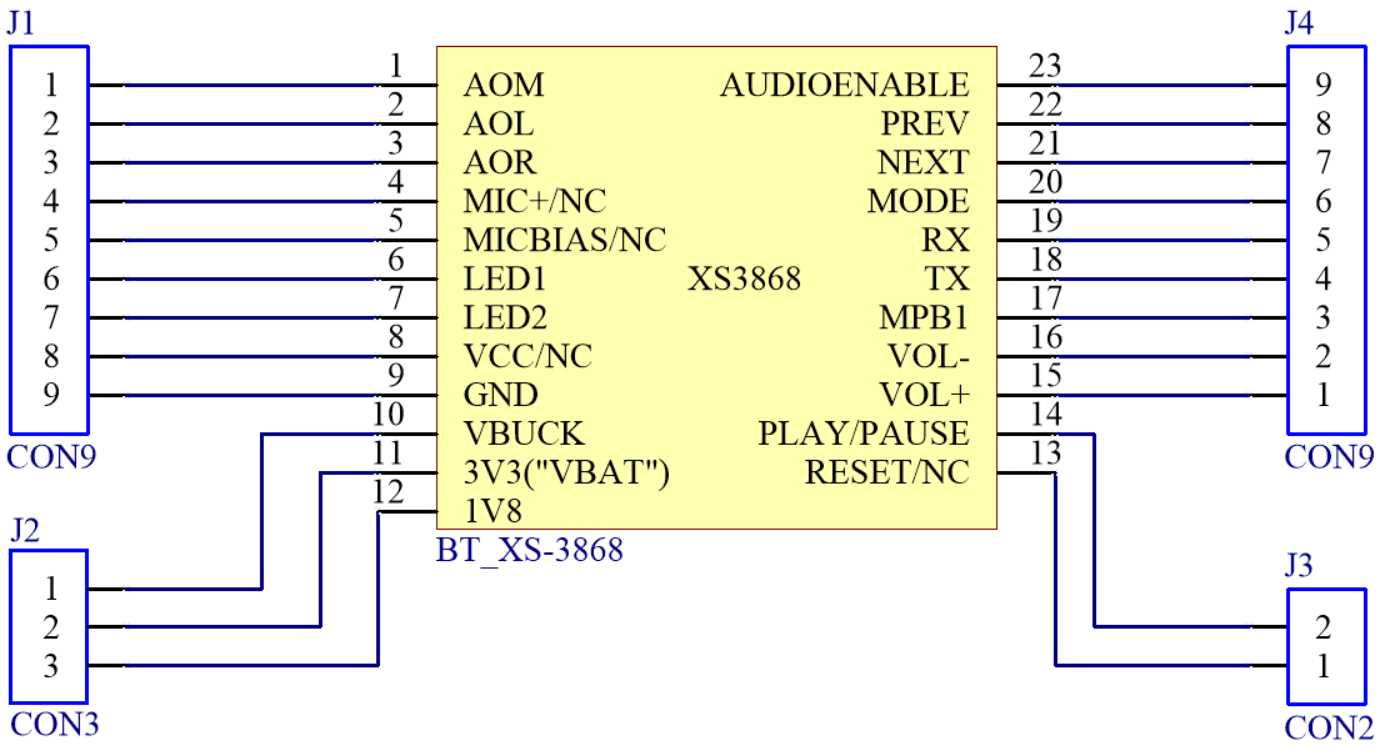
\includegraphics[width=1\textwidth]{schaltungen/adapter_sch.png}
\end{figure} \\
Jeder Pin bekommt auch auf dem Adapter einen eigenen Pin auf der Stiftleiste.
\newpage
Das PCB (Abb. \ref{fig:abb3.2}) ist, wie bereits erwähnt, einseitig aufgebaut:
\begin{figure} [h]
	\centering
	\caption{PCB des Adapter-Boards}
%%	\label {fig:abb3.2}
%%	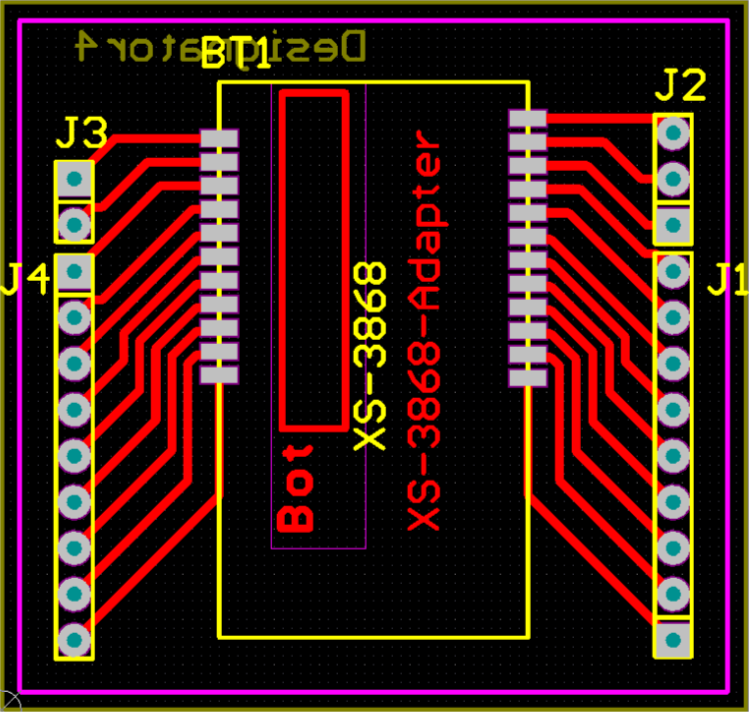
\includegraphics[width=1\textwidth]{schaltungen/adapter_pcb.png}
\end{figure} \\
Mit diesem PCB kann da BT-Modul nun besser getestet und auch weiterverwendet werden. Gemeinsam mit diesem Adapter kommt es auch auf das Hauptboard.
\newpage


\subsubsection{Hauptboard}
\minisec{Funktion}
Das Hauptboard wird hauptsächlich zur Versorgung des BT-Moduls, aber auch zur Weiterverarbeitung des Audio-Signals verwendet. Darüber hinaus ist eine Additionsschaltung vorgesehen, die das Signal des BT-Moduls mit einem zweiten, von einem Klinken-Eingang zugeführten, Signal vermischt. Die Lautstärke von diesem zweiten Audio-Signal kann über ein Stereo-Potentiometer geregelt werden. \\
Weiterhin sind die Pins zur Bedienung der Musik an einen 2x5-Wannenstecker herausgeführt. Zugang zur seriellen Schnittstelle wird auch ermöglicht.

\minisec{Schaltung}
Die Schaltung (Abb. \ref{fig:abb3.3}) des Hauptboards ist in mehrere Teile aufgeteilt und wird deshalb auch einzeln erklärt.
\begin{figure} [h]
	\centering
	\caption{Schaltung des Hauptboards (Versorgung + BT-Modul)}
%%	\label {fig:abb3.3}
%%	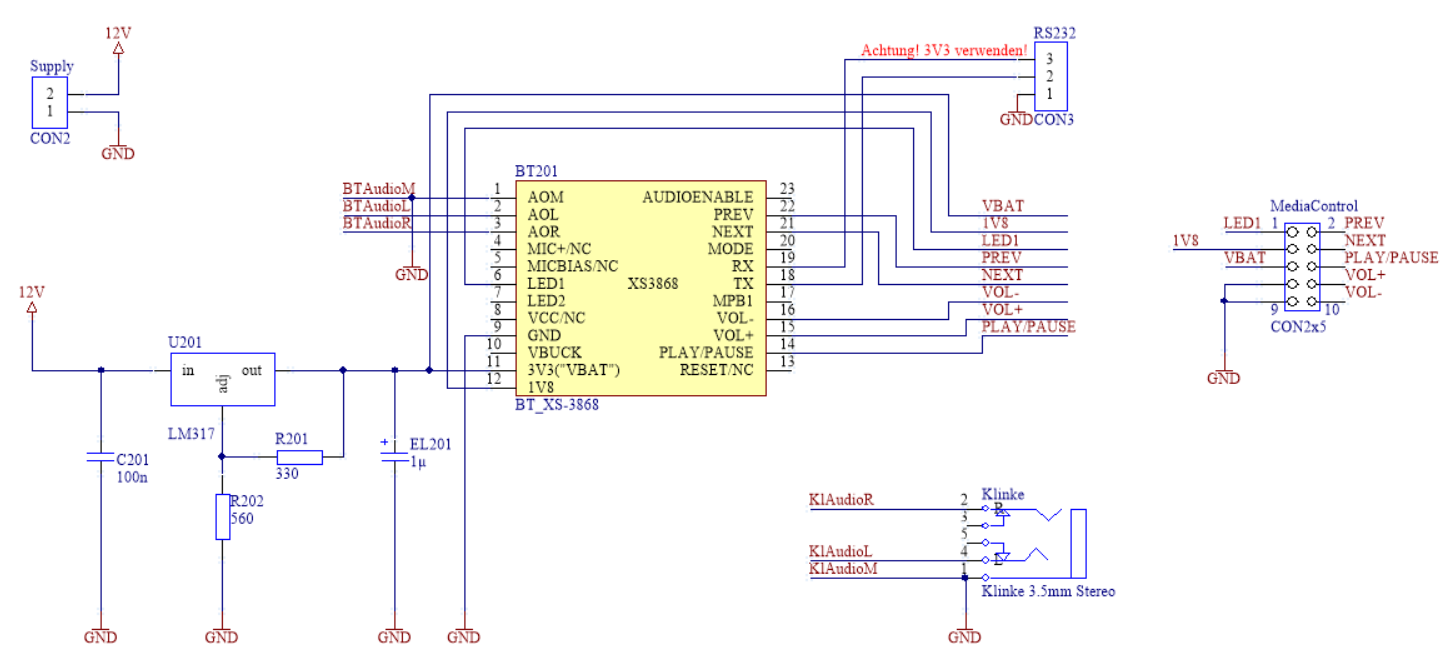
\includegraphics[width=1\textwidth]{schaltungen/hauptboard_sch1.png}
\end{figure} \\
In diesem Teil der Schaltung ist zu sehen: die Versorgungsbuchse, die Versorgungsschaltung für das BT-Modul, das BT-Modul mit herausgeführten Pins und die Klinken-Buchse.\\
Der Spannungsregler LM317 (Bezeichnung: U201) stellt eine Versorgungsspannung von 3,9V für das BT-Modul ein. Mit einer maximalen Stromaufnahme von 100mA ergibt sich folgende Verlustleistung:
\begin{equation}
	P_{max} = 7,9V * 100mA = 0,79W
\end{equation}
Deshalb wird auch kein Kühlkörper benötigt, es wird aber trotzdem eine Alu-Platte an den LM317 geschraubt um sicher zu gehen. \\
Ein eigener Stecker (Stiftleiste) für die Versorgung (12V) sowie die UART-Schnittstelle (RS232) sind auch vorgesehen. Der Wannenstecker (hier: \enquote{MediaControl}) ist mit allen wichtigen Pins des Moduls verbunden und verbindet eine Frontplatine mit dem Hauptboard. \\ \\
Die Klinkenbuchse wird in der folgenden Additionsschaltung(Abb. \ref {fig:abb3.4}) weiterverwendet:
\begin{figure} [h]
	\centering
	\caption{Schaltung des Hauptboards (Additionsschaltung)}
%%	\label {fig:abb3.4}
%%	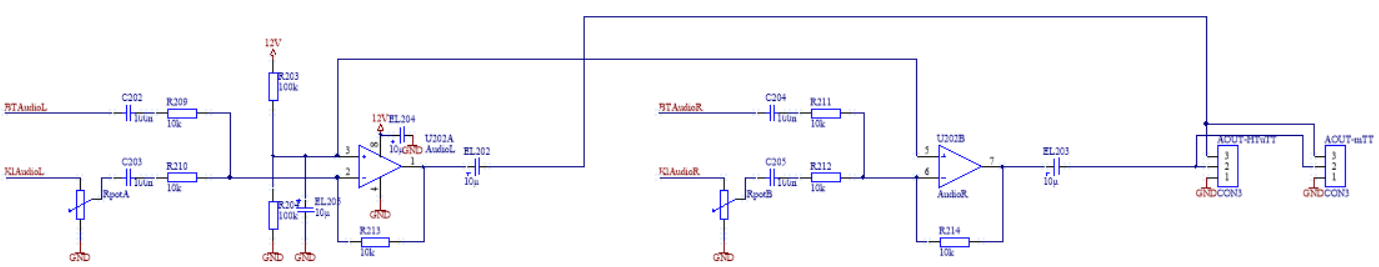
\includegraphics[width=1\textwidth]{schaltungen/hauptboard_sch2.png}
\end{figure} \\
Vergrößert:
\begin{figure} [h]
	\centering
	\caption{Schaltung des Hauptboards (linker Teil der Additionsschaltung)}
%%	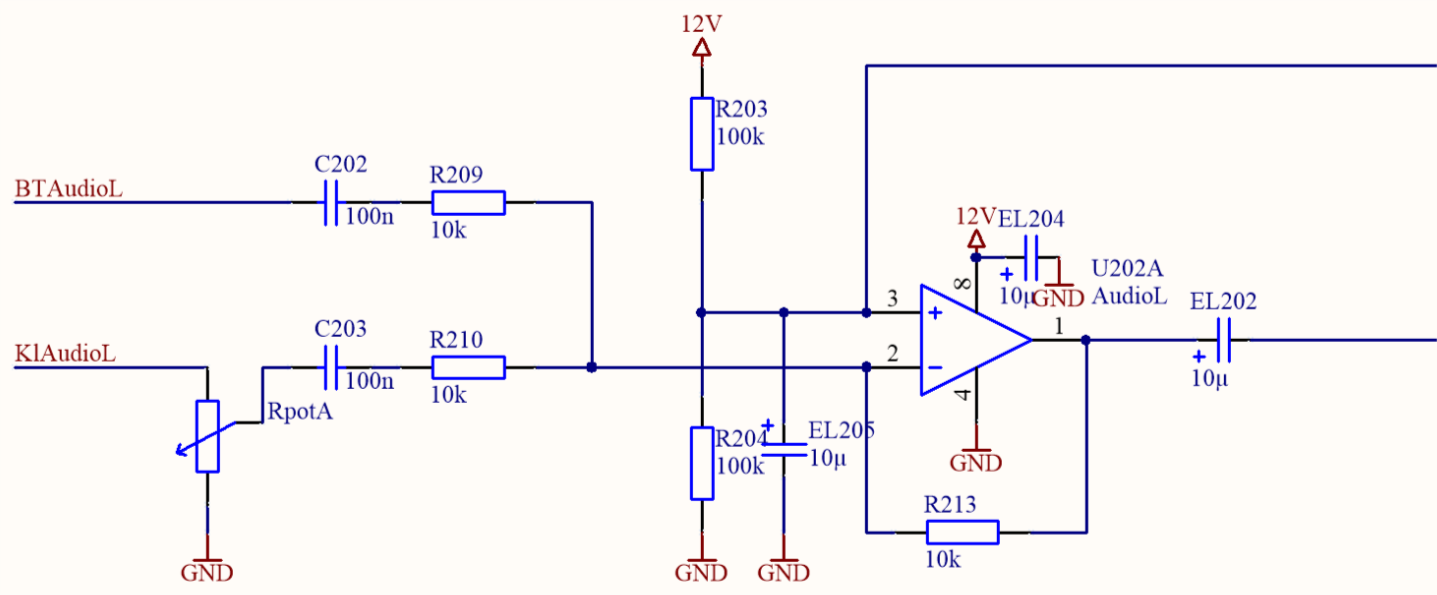
\includegraphics[width=1\textwidth]{schaltungen/hauptboard_sch2_zoom.png}
\end{figure} \\
Mithilfe dieser OPV-Schaltung werden die zwei Audio-Signale (ein Addierer pro Kanal) addiert. Das Signal vom Klinkeneingang kann zuvor noch mit einem Potentiometer abgeschwächt werden.\\
Der Arbeitspunkt bei 6V am Pin 3 wird benötigt um am Ausgang eine Spannung von $\pm$6V zu erreichen. Der OPV wird hier als invertierender Verstärker mit Verstärkung 1 aufgebaut, aber er addiert hier die zwei Signale zusammen auf ein Ausgangssignal.

\minisec{PCB}
Die Platine(Abb. \ref {fig:abb3.6}) für das Hauptboard sollte möglichst kompakt sein und alle Eingänge oder Bedienelemente auf einer Seite (hier rechts) haben. Das BT-Modul wird samt Adapter auf zwei Stiftleisten gesteckt. Darunter werden keine Bauteile verwendet, weil es sonst zu eng wäre. Des weiteren wären Bauteile unter dem Adapterprint während der Testphase unvorteilhaft, da diese schwerer zugänglich sind.
\begin{figure} [h]
	\centering
	\caption{PCB des Hauptboards}
%%	\label {fig:abb3.6}
	%%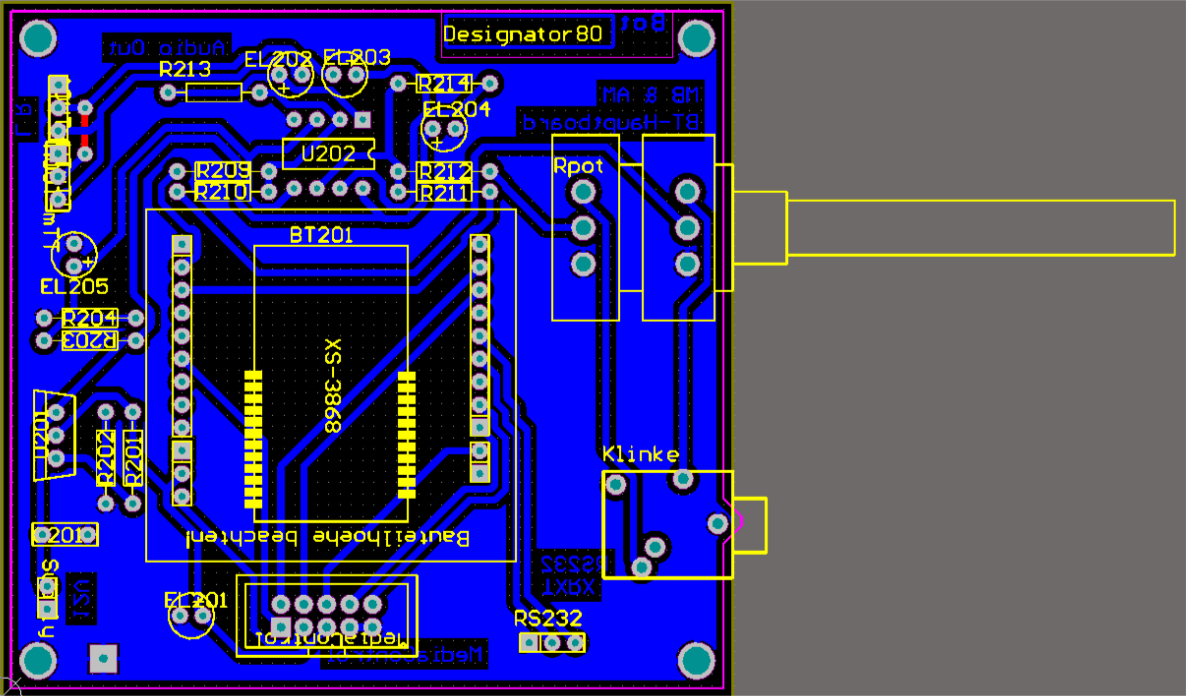
\includegraphics[width=1\textwidth]{schaltungen/hauptboard_pcb.png}
\end{figure}
\newpage


\subsubsection{Frontplatine}
\minisec{Funktion}
Diese Platine ist eigentlich eine Erweiterung des Hauptboards. Es wird mit dem Hauptboard über einen 2x5-Wannenstecker verbunden und auch versorgt. Sonst sind nur die Taster zur Bedienung des BT-Moduls, sowie die Status-LED verbaut.

\minisec{Schaltung}
Die Taster werden jeweils mithilfe eines Kondensators entprellt. Die Höhe der Taster reicht über die Kondensatoren hinaus um eine Bedienung zu ermöglichen. (Abb. \ref{fig:abb3.7})
\begin{figure} [h]
	\centering
	\caption{Schaltung der Frontplatine}
%%	\label {fig:abb3.7}
	%%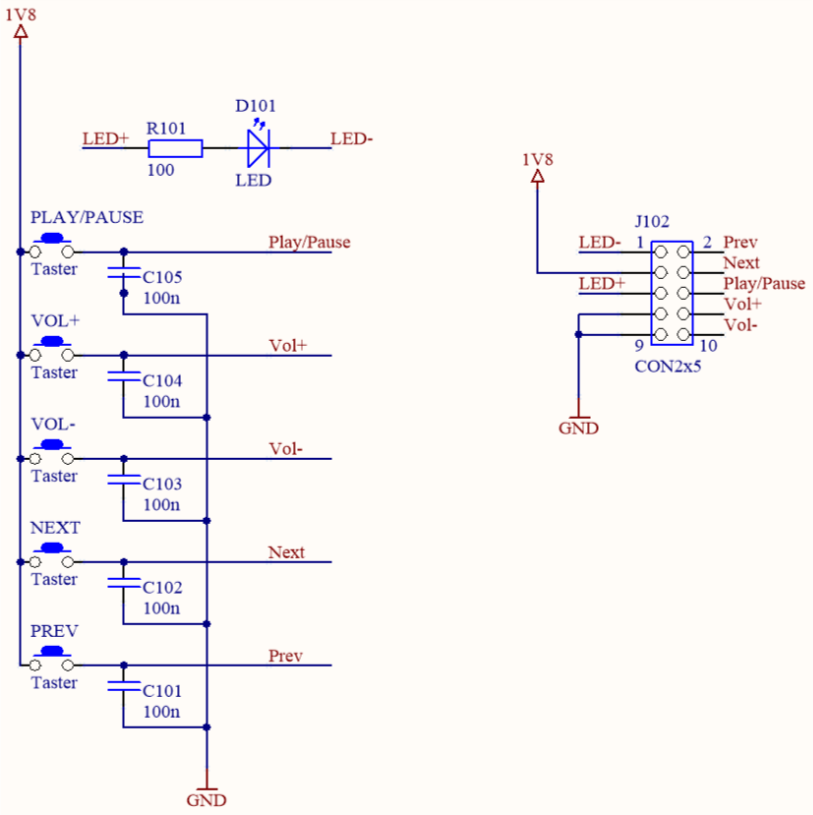
\includegraphics[width=0.7\textwidth]{schaltungen/front_sch.png}
\end{figure} \\
Jeder der Taster ist mit dem 1,8V-Pin des Moduls verbunden und geht dann weiter auf den entsprechenden Funktionspin. Die Bezeichnung \enquote{LED+} entspricht der Versorgungsspannung (\enquote{VBAT} = 3,9V) des Moduls. \enquote{LED-} ist mit dem Ansteuerungssignal am BT-Modul verbunden (Pin 6).

\minisec{PCB}
Das PCB (Abb. \ref {fig:abb3.8}) der Frontplatine soll ebenfalls so klein wie möglich aber von der Bedienung her sinnvoll aufgebaut sein.
\begin{figure} [h]
	\centering
	\caption{PCB der Frontplatine}
%%	\label {fig:abb3.8}
	%%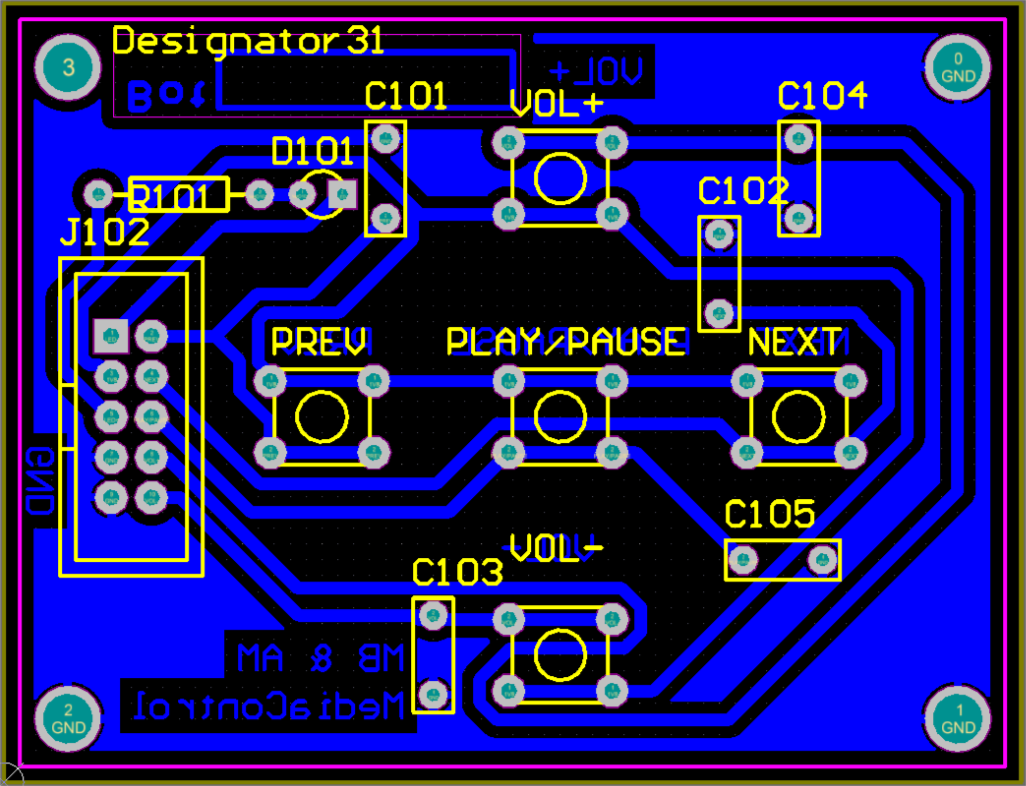
\includegraphics[width=1\textwidth]{schaltungen/front_pcb.png}
\end{figure} \\
Die Taster wurden in einem Kreuz aufgebaut, wobei an der linken oberen Ecke die Status-LED verbaut wurde.
\end{comment}






